\documentclass[10pt,UTF8]{ctexart}


\usepackage[margin=2cm,a4paper]{geometry}
%\usepackage[left=0.75in,top=0.6in,right=0.75in,bottom=1.0in,a4paper]{geometry}

\setmainfont{Caladea}
%% 也可以選用其它字庫:
% \setCJKmainfont[%
%   ItalicFont=AR PL KaitiM GB,
%   BoldFont=Noto Sans CJK SC,
% ]{Noto Serif CJK SC}
% setCJKsansfont{Noto Sans CJK SC}
% \renewcommand{\kaishu}{\CJKfontspec{AR PL KaitiM GB}}

% 繁體中文
\setCJKmainfont[Path=fonts/ ]{NotoSansTC-Medium.otf}

\usepackage{minted}
\usepackage[breaklinks]{hyperref}

% Picture
% 導言區的此三行無變化
\usepackage{graphicx}
\usepackage{float} 
\usepackage{subfigure}
% 以下是新增的自定義格式更改
\usepackage[]{caption2} %新增調用的宏包
\renewcommand{\figurename}{Fig.} %重定義編號前綴詞
\renewcommand{\captionlabeldelim}{.~} %重定義分隔符
 %\roman 是羅馬數字編號,\alph是默認的字母編號,\arabic是阿拉伯數字編號,可按需替換下一行的相應位置
\renewcommand{\thesubfigure}{(\roman{subfigure})}%此外,還可設置圖編號顯示格式,加括號或者不加括號
\makeatletter \renewcommand{\@thesubfigure}{\thesubfigure \space}%子圖編號與名稱的間隔設置
\renewcommand{\p@subfigure}{} \makeatother

% Math
\usepackage {mathtools}
\usepackage{amssymb}

% Code
\usepackage{listings}
\usepackage{xcolor}
\lstset{
    % backgroundcolor=\color{red!50!green!50!blue!50},
    % 程式碼塊背景色為淺灰色
    rulesepcolor= \color{gray}, % 程式碼塊邊框顏色
    breaklines=true,  % 程式碼過長則換行
    numbers=left, % 行號在左側顯示
    numberstyle= \small,% 行號字型
    % eywordstyle= \color{red,% 關鍵字顏色
    commentstyle=\color{gray}, % 註釋顏色
    frame=shadowbox % 用方框框住程式碼塊
    }

\usepackage{hyperref}

\title{算法分析和複雜性理論}
\author{干皓丞,2101212850, 信息工程學院}

\begin{document}
\maketitle


\section{作業目標與章節摘要}

1. LeetCode 7. Reverse Integer 整數反轉

2. LeetCode 13. Roman to Integer 羅馬數字轉整數

3. LeetCode 66. Plus One 加一

4. 本地終端測試調研

5. 前次課堂練習,與問題紀錄

\section{作業內容概述}

作業可以從 GitHub 下的 kancheng/kan-cs-report-in-2022 專案找到,作業程式碼與文件目錄為 kan-cs-report-in-2022/AATCC/lab-report/w1。實際執行的環境與實驗設備為 Google 的 Colab 、MacBook Pro (Retina, 15-inch, Mid 2014) 、 Acer Aspire R7 與 HP Victus (Nvidia GeForce RTX 3060)。

本作業 GitHub 專案為 kancheng/kan-cs-report-in-2022 下的 AATCC` 的目錄。程式碼可以從 code 目錄下可以找到 *.pynb,內容包含上次課堂練習、LeetCode 範例思路整理與作業,最後包含其他語言範例。

https://github.com/kancheng/kan-cs-report-in-2022/tree/main/AATCC

\begin{figure}[H]
\centering 

\includegraphics[width=0.30\textwidth]{aatccqr.png} 
\caption{作業專案位置}
\label{Test}
\end{figure}


1. LeetCode : https://leetcode.com/

2. LeetCode CN : https://leetcode-cn.com/

3. OnlineGDB : https://www.onlinegdb.com/ 

LeetCode 的平台部分, CN 的平台有針對簡體中文使用者進行處理,包含中英文切換等功能。OnlineGDB 則可線上進行簡易的環境測試,其程式碼涵蓋 C, C++, C\#, Java, Python, JS, Rust, Go。

\newpage

\section{LeetCode 7. Reverse Integer 整數反轉}

\subsection{LeetCode 7. 題目}

Given a signed 32-bit integer x, return x with its digits reversed. If reversing x causes the value to go outside the signed 32-bit integer range $[-2^{31}, 2^{31} - 1]$, then return 0.

Assume the environment does not allow you to store 64-bit integers (signed or unsigned).


給你一個 32 位的有符號整數 x ,返回將 x 中的數字部分反轉後的結果。

如果反轉後整數超過 32 位的有符號整數的範圍 $[−2^{31}, 2^{31} − 1]$ ,就返回 0。

假設環境不允許存儲 64 位整數(有符號或無符號)。

給定一個整數數組 nums 和一個整數目標值 target,請你在該數組中找出 和為目標值 target  的那 兩個 整數,並返回它們的數組下標。

你可以假設每種輸入只會對應一個答案。但是,數組中同一個元素在答案裡不能重複出現。

你可以按任意順序返回答案。

Example 1:
\begin{lstlisting}[language={python}]
Input: x = 123
Output: 321
\end{lstlisting}

Example 2:
\begin{lstlisting}[language={python}]
Input: x = -123
Output: -321
\end{lstlisting}

Example 3:
\begin{lstlisting}[language={python}]
Input: x = 120
Output: 21
\end{lstlisting}

\subsection{LeetCode 7. 思路總結}


1. 要求反轉 10 進位。

2. 其反轉的數字必須在 $[−2^31, 2^31 − 1]$ 範圍內,若超過範圍則必須輸出 0 。

\subsection{LeetCode 7. Code 範例}

LeetCode 7. Python 1 \& 2

\begin{lstlisting}[language={python}]
# 絕對值
class Solution1:
    def reverse(self, x: int) -> int:
        max_32 = 2 ** 31 - 1
        if abs(x) > max_32:
            return 0
        if x < 0:
            rint = -int(str(abs(x))[::-1])
        else:
            rint = int(str(x)[::-1])
        if abs(rint) > max_32:
            return 0
        else:
            return rint 
x1 = -123
x2 = 123
x3 = 120
ob1 = Solution1()
print(ob1.reverse(x1))
print(ob1.reverse(x2))
print(ob1.reverse(x3))
# 字串
class Solution2:
    def reverse(self, x):
        """
        :type x: int
        :rtype: int
        """
        if x==0:
            return 0
        str_x = str(x)
        x = ''
        if str_x[0] == '-':
            x += '-'
        x += str_x[len(str_x)-1::-1].lstrip("0").rstrip("-")
        x = int(x)
        if -2**31<x<2**31-1:
            return x
        return 0
x1 = -123
x2 = 123
x3 = 120
ob2 = Solution2()
print(ob2.reverse(x1))
print(ob2.reverse(x2))
print(ob2.reverse(x3))
\end{lstlisting}

\subsection{LeetCode 7. 結果}

\begin{figure}[H]
\centering 
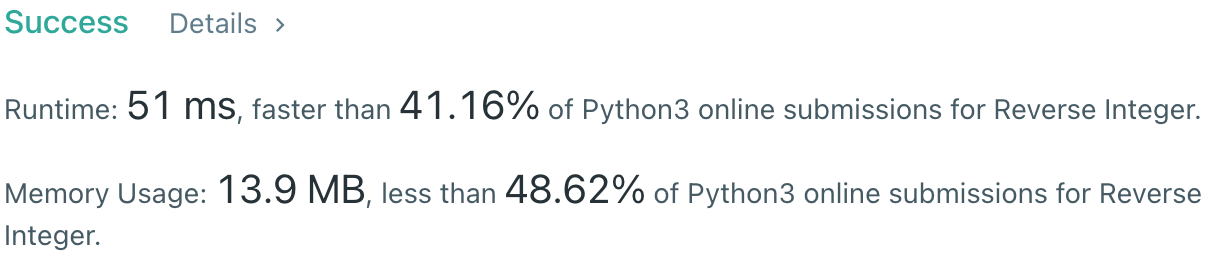
\includegraphics[width=0.80\textwidth]{lc-7-1.png} 
\caption{LeetCode 7 第一個範例結果}
\label{Test}
\end{figure}

\begin{figure}[H]
\centering 
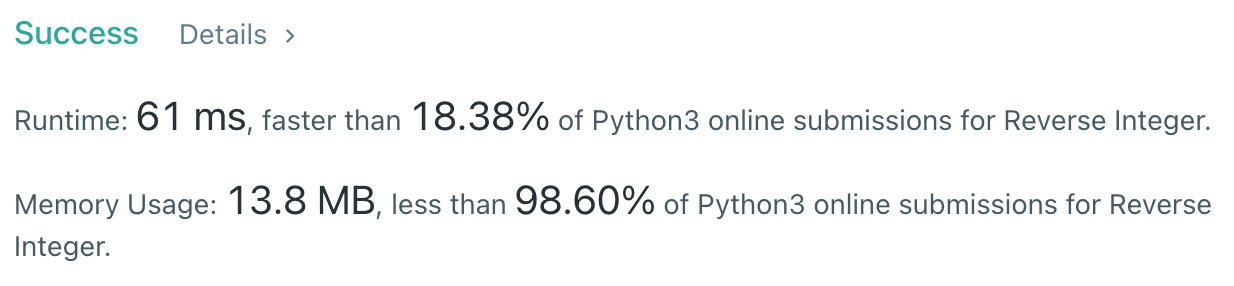
\includegraphics[width=0.80\textwidth]{lc-7-2.png} 
\caption{LeetCode 7 第二個範例結果}
\label{Test}
\end{figure}

\subsection{LeetCode 7. 終端效能測試}

\begin{lstlisting}[language={python}]
(base) HaoyeMacBookPro:w2 kancheng$ python lc-7-test.py 
-321
321
21
Process Time: time of EX 1 is 0.00008
-321
321
21
Perf Counter: time of EX 1 is 0.00002
-321
321
21
Process Time: time of EX 2 is 0.00003
-321
321
21
Perf Counter: time of EX 2 is 0.00002
(base) HaoyeMacBookPro:w2 kancheng$ 
\end{lstlisting}

\newpage

\section{LeetCode 13. Roman to Integer 羅馬數字轉整數}

\subsection{LeetCode 13. 題目}

Roman numerals are represented by seven different symbols: I, V, X, L, C, D and M.

```
Symbol       Value
I             1
V             5
X             10
L             50
C             100
D             500
M             1000
```

For example, 2 is written as II in Roman numeral, just two one's added together. 

12 is written as XII, which is simply X + II. 

The number 27 is written as XXVII, which is XX + V + II.

Roman numerals are usually written largest to smallest from left to right. 

However, the numeral for four is not IIII. 

Instead, the number four is written as IV. 

Because the one is before the five we subtract it making four. 

The same principle applies to the number nine, which is written as IX. There are six instances where subtraction is used:

I can be placed before V (5) and X (10) to make 4 and 9.
X can be placed before L (50) and C (100) to make 40 and 90.
C can be placed before D (500) and M (1000) to make 400 and 900.
Given a roman numeral, convert it to an integer.

羅馬數字包含以下七種字符: I, V, X, L,C,D 和 M。

例如, 羅馬數字 2 寫做 II ,即為兩個並列的 1 。 12 寫做 XII ,即為 X + II 。 27 寫做 XXVII, 即為 XX + V + II 。

通常情況下,羅馬數字中小的數字在大的數字的右邊。但也存在特例,例如 4 不寫做 IIII,而是 IV。數字 1 在數字 5 的左邊,所表示的數等於大數 5 減小數 1 得到的數值 4 。同樣地,數字 9 表示為 IX。這個特殊的規則只適用於以下六種情況:

I 可以放在 V (5) 和 X (10) 的左邊,來表示 4 和 9。

X 可以放在 L (50) 和 C (100) 的左邊,來表示 40 和 90。

C 可以放在 D (500) 和 M (1000) 的左邊,來表示 400 和 900。

給定一個羅馬數字,將其轉換成整數。


Example 1:
\begin{lstlisting}[language={python}]
Input: s = "III"
Output: 3
Explanation: III = 3.
\end{lstlisting}

Example 2:
\begin{lstlisting}[language={python}]
Input: "IV"
Output: 4
\end{lstlisting}

Example 3:
\begin{lstlisting}[language={python}]
Input: "IX"
Output: 9
\end{lstlisting}

Example 4:
\begin{lstlisting}[language={python}]
Input: "LVIII"
Output: 58
Explanation: L = 50, V= 5, III = 3.
\end{lstlisting}

Example 5:
\begin{lstlisting}[language={python}]
Input: "MCMXCIV"
Output: 1994
Explanation: M = 1000, CM = 900, XC = 90 and IV = 4.
\end{lstlisting}

Constraints:

- 1 <= s.length <= 15

- s contains only the characters ('I', 'V', 'X', 'L', 'C', 'D', 'M').

s 僅含字符 ('I', 'V', 'X', 'L', 'C', 'D', 'M')

- It is guaranteed that s is a valid roman numeral in the range $[1, 3999]$.

題目數據保證 s 是一個有效的羅馬數字,且表示整數在範圍 $[1, 3999]$ 內

題目所給測試用例皆符合羅馬數字書寫規則,不會出現跨位等情況。 IL 和 IM 這樣的例子並不符合題目要求,49 應該寫作 XLIX,999 應該寫作 CMXCIX 。關於羅馬數字的詳盡書寫規則,可以參考 羅馬數字 - Mathematics 。

https://b2b.partcommunity.com/community/knowledge/en/detail/10753/Roman\%20numerals

\subsection{LeetCode 13. 思路總結}

1. 給一個羅馬數字,將其轉換成整數。其輸入確保在 1 ~ 3999 的範圍內。

2. 按要求的羅馬數字計算出對應的 10 進位阿拉伯數字即可。

3. 首先建立一個 HashMap 或者是 Python 的字典來抓相對應的符號與值,而後對字串從左至右來處理。若當前字符代表的值不小於右邊,就加上該值;否則就减去該值。類推到最左邊的數。

\subsection{LeetCode 13. Code 範例}

\begin{lstlisting}[language={python}]
class Solution1:
    def romanToInt(self, s):
        rn = {'I':1, 'V':5, 'X':10, 'L':50, 'C':100, 'D':500, 'M':1000}        
        ans=0        
        for i in range(len(s)):            
            if i<len(s)-1 and rn[s[i]]<rn[s[i+1]]:                
                ans -= rn[s[i]]
            else:
                ans += rn[s[i]]
        return ans
x = "III"
ob1 = Solution1()
print(ob1.romanToInt(x))
class Solution2:
    def romanToInt(self, s: 'str') -> 'int':
        value_roman = {"M":1000, "CM":900, "D":500, "CD": 400,
                       "C":100,"XC":90, "L":50, "XL":40,
                       "X":10, "IX":9, "V":5, "IV":4, "I":1}
        num = 0
        specials_list = ["CM","CD","XC","XL","IX","IV"]
        for i in specials_list:
            if i in s:
                num = num + value_roman[i]
                s=s.replace(i,"")
        for i in s:
            num = num + value_roman[i]
        return(num)
x = "III"
ob2 = Solution2()
print(ob2.romanToInt(x))
\end{lstlisting}

\subsection{LeetCode 13. 結果}

\begin{figure}[H]
\centering 
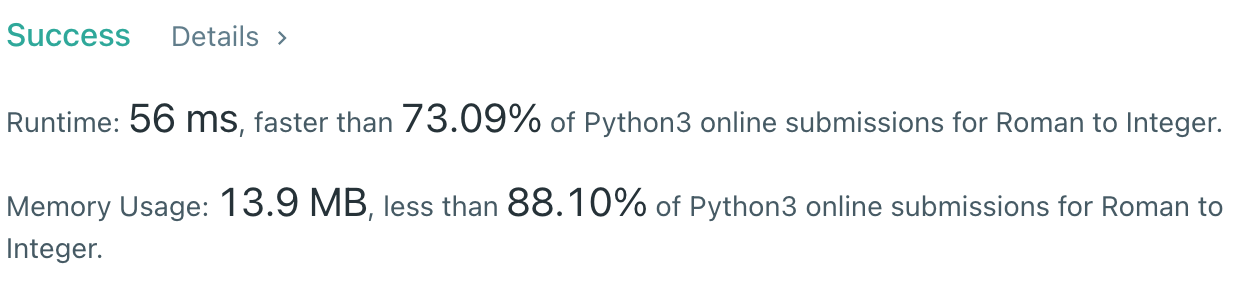
\includegraphics[width=0.80\textwidth]{lc-13-1.png} 
\caption{LeetCode 13 第一個範例結果}
\label{Test}
\end{figure}

\begin{figure}[H]
\centering 
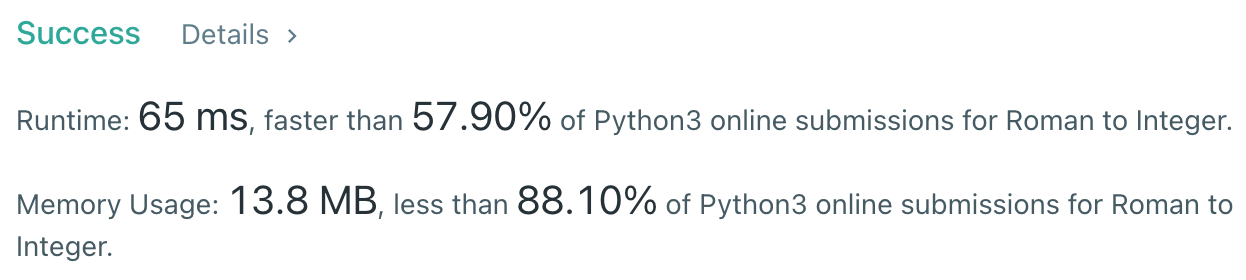
\includegraphics[width=0.80\textwidth]{lc-13-2.png} 
\caption{LeetCode 13 第二個範例結果}
\label{Test}
\end{figure}

\subsection{LeetCode 13. 終端效能測試}

\begin{lstlisting}[language={python}]
(base) HaoyeMacBookPro:w2 kancheng$ python lc-13-test.py 
3
Process Time: time of EX 1 is 0.00008
3
Perf Counter: time of EX 1 is 0.00002
3
Process Time: time of EX 2 is 0.00002
3
Perf Counter: time of EX 2 is 0.00002
(base) HaoyeMacBookPro:w2 kancheng$ 
\end{lstlisting}

\newpage

\section{LeetCode 66. Plus One 加一}

\subsection{LeetCode 66. 題目}

You are given a large integer represented as an integer array digits, where each digits[i] is the $i^{th}$ digit of the integer. 

The digits are ordered from most significant to least significant in left-to-right order. 

The large integer does not contain any leading 0's.

Increment the large integer by one and return the resulting array of digits.

給定一個由 整數 組成的 非空 數組所表示的非負整數,在該數的基礎上加一。

最高位數字存放在數組的首位, 數組中每個元素只存儲單個數字。

你可以假設除了整數 0 之外,這個整數不會以零開頭。

Example 1:
\begin{lstlisting}[language={python}]
Input: digits = [1,2,3]
Output: [1,2,4]
Explanation: The array represents the integer 123.
Incrementing by one gives 123 + 1 = 124.
Thus, the result should be [1,2,4].
\end{lstlisting}

Example 2:
\begin{lstlisting}[language={python}]
Input: digits = [4,3,2,1]
Output: [4,3,2,2]
Explanation: The array represents the integer 4321.
Incrementing by one gives 4321 + 1 = 4322.
Thus, the result should be [4,3,2,2].
\end{lstlisting}

Example 3:
\begin{lstlisting}[language={python}]
Input: digits = [9]
Output: [1,0]
Explanation: The array represents the integer 9.
Incrementing by one gives 9 + 1 = 10.
Thus, the result should be [1,0].
\end{lstlisting}

Constraints:

1. 1 <= digits.length <= 100
2. 0 <= digits[i] <= 9
3.  digits does not contain any leading 0's.

\subsection{LeetCode 66. 思路總結}

1. 給一個陣列(数组, Array),代表一個十進位數,陣列的 0 下標是十進位數的高位。要求計算這個十進位數加一以後的結果。

2. 從陣列尾部開始由後往前掃,逐位進位即可。最高位若還有進位的需要則在數組內第 0 位再插入一個 1。

\subsection{LeetCode 66. Code 範例}

\begin{lstlisting}[language={python}]
from typing import List
class Solution1:
    def plusOne(self, digits: List[int]) -> List[int]:
        h = ''.join(map(str, digits))
        h = str(int(h) + 1)
        output = []
        for ch in h:
            output.append(int(ch))
        return output
x = [1,2,3]
ob1 = Solution1()
print(ob1.plusOne([1,2,3]))
class Solution2:
    def plusOne(self, digits: List[int]) -> List[int]:
        return list(map(int, list(str(int(''.join(map(str, digits))) + 1))))
x = [1,2,3]
ob2 = Solution2()
print(ob2.plusOne([1,2,3]))
\end{lstlisting}

\subsection{LeetCode 66. 結果}

\begin{figure}[H]
\centering 
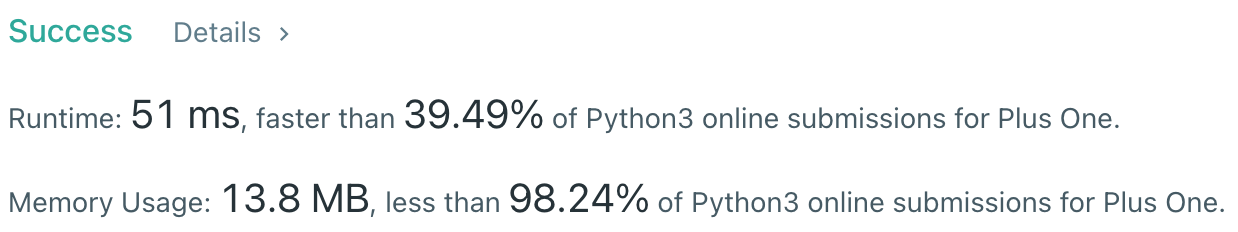
\includegraphics[width=0.80\textwidth]{lc-66-1.png} 
\caption{LeetCode 66 第一個範例結果}
\label{Test}
\end{figure}

\begin{figure}[H]
\centering 
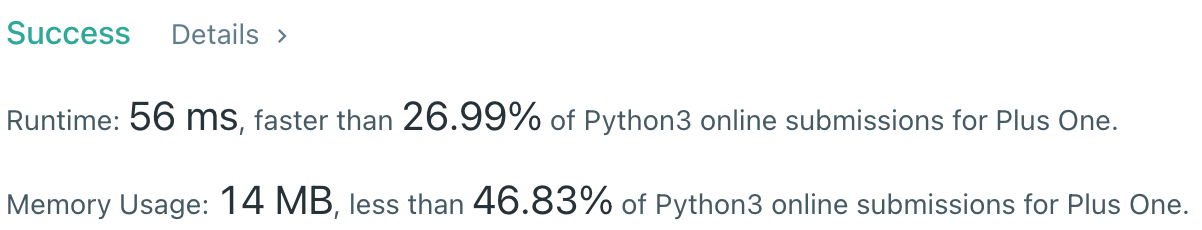
\includegraphics[width=0.80\textwidth]{lc-66-2.png} 
\caption{LeetCode 66 第二個範例結果}
\label{Test}
\end{figure}

\subsection{LeetCode 66. 終端效能測試}

\begin{lstlisting}[language={python}]
(base) HaoyeMacBookPro:w2 kancheng$ python lc-66-test.py 
[1, 2, 4]
Process Time: time of EX 1 is 0.00010
[1, 2, 4]
Perf Counter: time of EX 1 is 0.00003
[1, 2, 4]
Process Time: time of EX 2 is 0.00002
[1, 2, 4]
Perf Counter: time of EX 2 is 0.00002
(base) HaoyeMacBookPro:w2 kancheng$
\end{lstlisting}

\newpage

\section{本地終端測試調研}

根據成功大學 Linux 系統設計與實作,整理出測試方案。

1. Linux Perf : https://perf.wiki.kernel.org/index.php/Main\_Page

2. Cppcheck : https://cppcheck.sourceforge.io/

3. Valgrind : https://github.com/LouisBrunner/valgrind-macos

4. Instruments

5. Google Perftools : https://github.com/gperftools/gperftools

6. Python Profilers 分析器 : https://docs.python.org/zh-cn/3.11/library/profile.html

7. Python timeit : https://docs.python.org/zh-tw/3/library/timeit.html

8. Python pympler : https://pympler.readthedocs.io/en/latest/

\subsection{Valgrind}

一般的方式無法對 Python 測試,不用讓腳本啟動解釋器,而是直接將其作為 Valgrind 的參數來解決該問題。

\begin{lstlisting}[language={python}]
valgrind --tool=memcheck --leak-check=full ./[File Name]
valgrind --tool=massif python [File Name].py
\end{lstlisting}

\section{前次課堂練習,與問題紀錄}

當中的簡報 time.clock() 問題,該程式碼在 Python 中被正式移除,其原因在於不同的作業系統的時間資料規範不一,其整理如下。


From the Python 3.8 doc:

The function time.clock() has been removed, after having been deprecated since Python 3.3: 

use time.perf\_counter() or time.process\_time() instead, depending on your requirements, to have well-defined behavior. (Contributed by Matthias Bussonnier in bpo-36895.)

time.clock()在 3.8 中被刪除,因為它具有平台相關的行為:

1. 在 Unix 上,這將返回當前處理器時間(以秒為單位)

2. 在 Windows 上,這將返回掛鐘時間(以秒為單位)

https://docs.python.org/3.7/library/time.html?highlight=time%20clock#time.clock

1. Processor Time: This is how long this specific process spends actively being executed on the CPU. Sleep, waiting for a web request, or time when only other processes are executed will not contribute to this.
處理器時間:這是該特定進程在 CPU 上主動執行所花費的時間。睡眠、等待 Web 請求或僅執行其他進程的時間不會對此產生影響。


(1) Use time.process\_time(), 採用 time.process\_time()


2. Wall-Clock Time: This refers to how much time has passed "on a clock hanging on the wall", i.e. outside real time.
掛鐘時間:這是指“掛在牆上的時鐘”已經過去了多少時間,即在實時之外。


(1) Use time.perf\_counter(), 採用 time.perf\_counter()


(A) time.time() also measures wall-clock time but can be reset, so you could go back in time
  time.time() 也測量掛鐘時間,但可以重置,所以你可以回到過去

(B) time.monotonic() cannot be reset (monotonic = only goes forward) but has lower precision than time.perf\_counter()
  time.monotonic() 無法重置(單調 = 僅向前)但精度低於time.perf\_counter()



%\section{附錄}

% 數學意義說明

% $$\min \limits_{G}\max \limits_{D}{V_I(D,\ G)=V(D,G)-\lambda L_I(G,Q)}$$

%	\begin{lstlisting}[language={python}]

%	\end{lstlisting}

%\begin{enumerate}
%\item Y
%\item A
%\end{enumerate}

% \newpage

\clearpage

\end{document}